\section{Introduction}

\note{jk: you need two paragraphs in intro to describe the problem statement.
	What I read in the first paragraph is not relevant with the problem that your
	thesis solves. The problem is: 1. Data analytics and search engines running on JVM need large heaps.
	2. A promising solution for large heaps that do not increase the GC cost is dual-heap designes, such as TeraHeap. Explain how does TeraHeap work and explain the problem of DRAM division.
	3. Then put a paragraph describing in high level your solution and how does this solution work.
	4. write where you implement your solution and provide some high-level results.
}


As modern applications such as \textbf{Apache Lucene}
\cite{klinaftakis2025thesis} and \textbf{Apache Spark}, grow in scale and
complexity, efficient memory management has become an important factor in
achieving optimal performance. Lucene performs intensive indexing and query
evaluation on large in-memory data structures such as a query cache, while
Spark continuously allocates and frees large volumes of temporary objects
during distributed computation. Both systems report highly dynamic memory
behavior, alternating between phases of high I/O and high GC creating an ideal
environment to apply a dynamic heap resizing policy.

The system used in this work is G1-TeraHeap, which as mentioned, is a dual
tiered memory management system, relying on a static DRAM configuration defined
at startup. A fixed DRAM partitioning assumes a uniform workload behavior
throughout execution. However, real-world applications frequently shift between
phases with different memory and I/O demands, leading to imbalanced DRAM usage
where budget remains underutilized leading to memory pressure, or increased
traffic. This mismatch can cause increased garbage  collection, I/O stalls,
ultimately degrading performance.

Moreover, Figure~\ref{fig:vanilla-dram-underutilization} illustrates a native
Lucene benchmark using a total of 8GB of DRAM, evenly split between H1 and the
OS page cache. At the beginning of the run, the heap usage rapidly spikes,
placing pressure on H1. As the benchmark execution progresses, the heap usage
stabilizes at a much lower level, suggesting that excess DRAM could be
reallocated to the page increasing it's capacity to read from the H2 file,
while reducing I/O produced by evictions, without massively affecting GC
performance. This behavior highlights the limitations of static partitioning
and motivates the need for a dynamic resizing mechanism that can react to
changes in workload phases.
\begin{figure}[htbp]
	\centering
	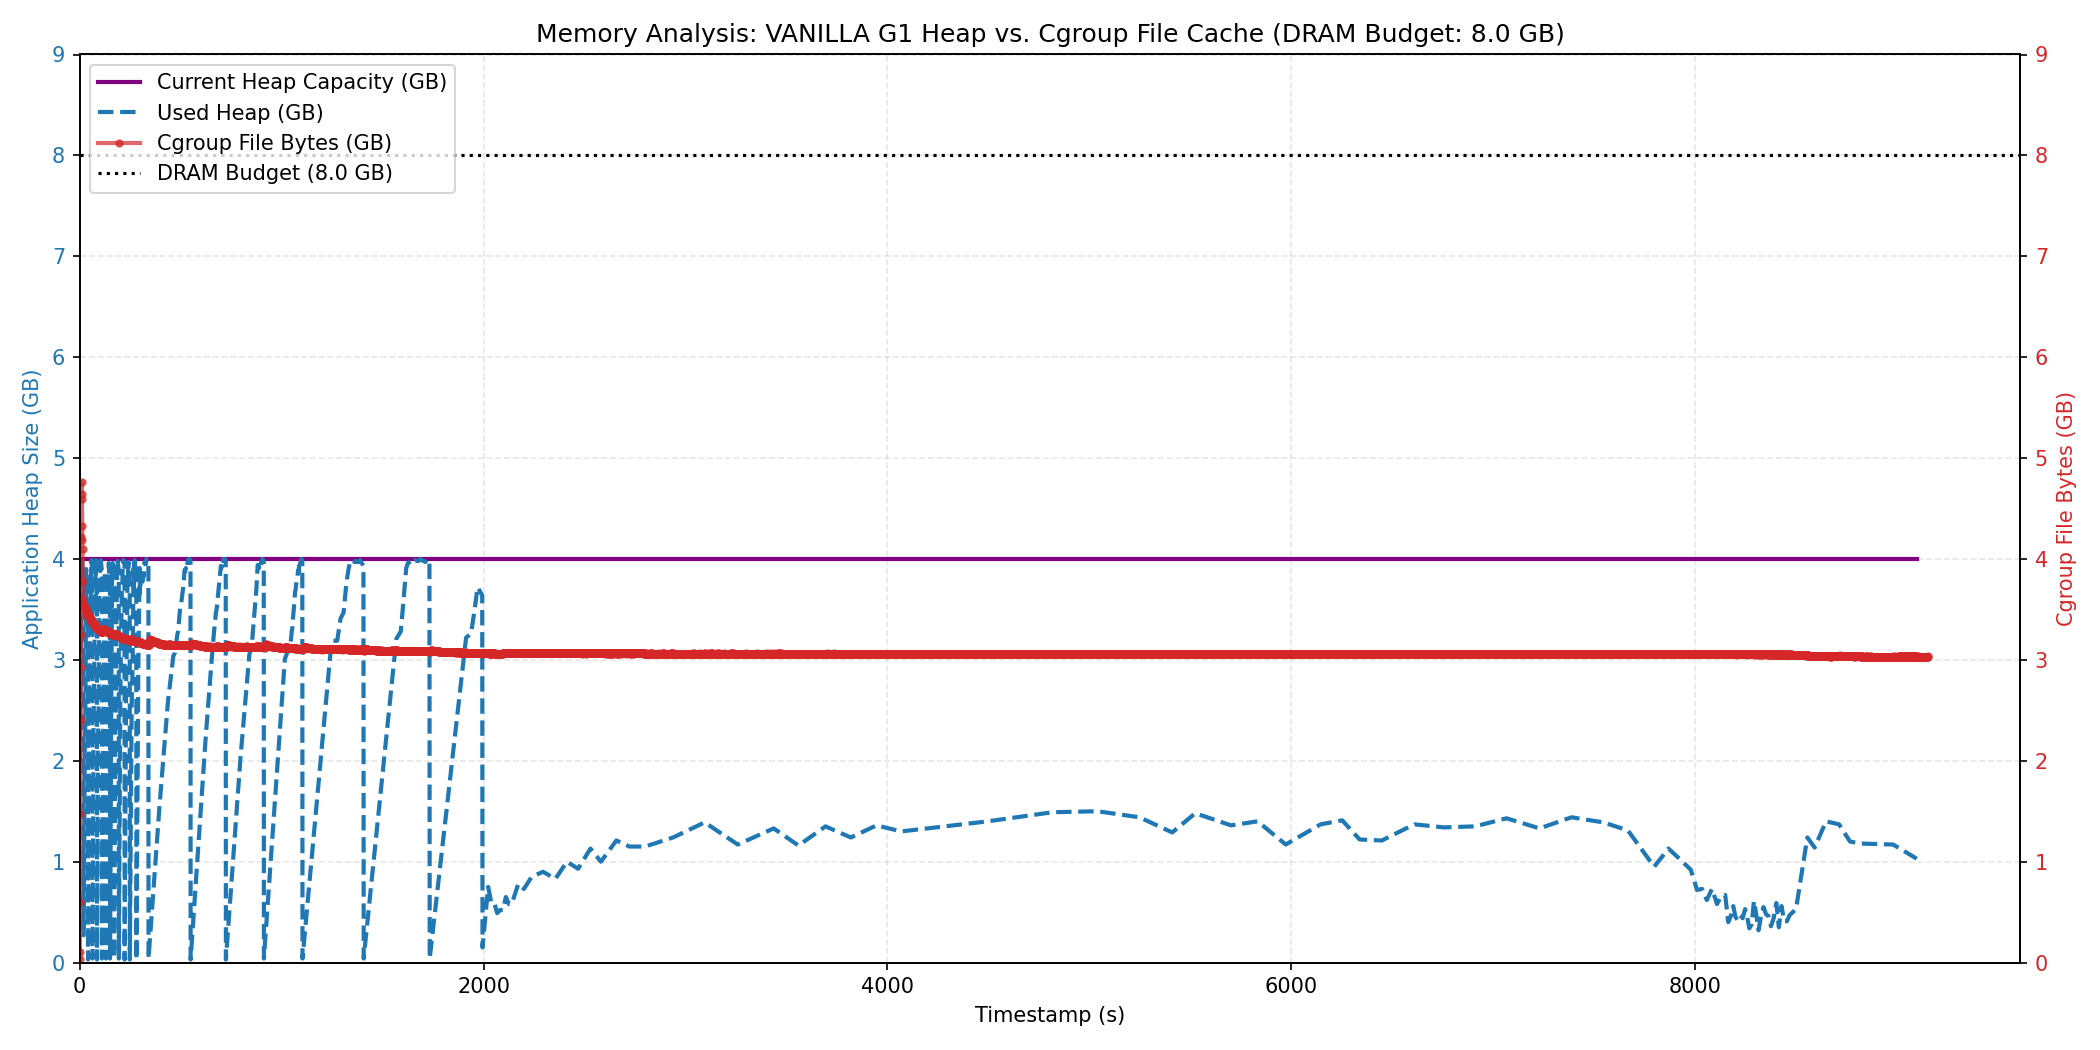
\includegraphics[width=1\linewidth]{fig/combined_memory_timeline_vanilla_g1.png}
	\caption{
		M1 Lucene benchmark with static DRAM configuration of 4GB H1 and 4GB pagecache.
	}
	\label{fig:vanilla-dram-underutilization}
\end{figure}

To address this limitation, we integrate \textbf{FlexHeap} to our system.
FlexHeap introduces a dynamic resizing policy that operates at runtime by
dividing execution into sampling intervals. During each interval, it tracks the
number of CPU cycles lost to GC (garbage collection) and the overheads from I/O
accesses to the remote heap (H2). At the end of the interval, it compares the
change in these two metrics relative to the previous intervals. If garbage
collection overhead has increased more than I/O stalls, more DRAM is
partitioned to H1 to relieve GC pressure, else if I/O delays have increased,
then the system shifts DRAM towards the pagecache to reduce evictions and hold
more data from the H2 file. This feedback-driven approach enables continuous
adaptation of the heap layout based on observed runtime behavior, ensuring that
the DRAM budget is effectively utilized.


